\SourceLeaf{168}succeed in overcoming every obstacle. I would then take the
greatest pleasure in doing everything in my power to see your achievement
recognized and brought to light. I now come
straight to the matter.

I have no substantial objection to any of the \textls{other} conclusions.
What has \textls{not} 
convinced me is just the reasoning in Article XIII. There you imagine
a line $\Pi\dots kdcfg\dots$ extended indefinitely,
consisting entirely of equal straight segments $kd$, $dc$, $cf$,
$fg$, etc., with the angles $kdc$, $dcf$, $cfg$, etc., equal to one another,
and you want to prove that $\Pi$ must sooner or later
pass beyond $k\varphi$. To this end you move the
straight line $kd\infty = Q$ toward the side on which $\Pi$ lies,
rotating it about $k$ so that it passes successively from one side of
the polygon $\Pi$ to the next. You show very well that $Q$,
as it passes in turn through $d, c, f, g$, etc., comes closer each time
to $k\varphi$. There is
\textls{Nothing} 
to object to in any of this. But then you continue
\begin{center}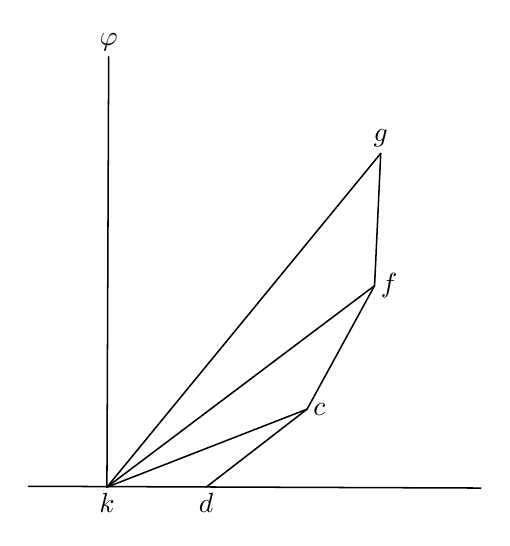
\begin{tikzpicture}[x=1.12cm,y=1.12cm,line width=.55pt,line cap=round,line join=round]
\coordinate (k) at (0,0);
\coordinate (d) at (1.125,0);
\coordinate (c) at (2.27,.885);
\coordinate (f) at (3.035,2.285);
\coordinate (g) at (3.105,3.785);
\coordinate (phi) at (.02,4.88);
\draw (-.89,.01)--(4.24,-.01);
\draw (k)--(phi);
\draw (k)--(c);
\draw (k)--(f);
\draw (k)--(g);
\draw (d)--(c)--(f)--(g);
\node[above,inner sep=2pt] at (phi) {$\varphi$};
\node[above,inner sep=2pt] at (g) {$g$};
\node[right,inner sep=2pt] at (f) {$f$};
\node[right,inner sep=2pt] at (c) {$c$};
\node[below,inner sep=2pt] at (d) {$d$};
\node[below,inner sep=2pt] at (k) {$k$};
\end{tikzpicture}
\end{center}
\begin{quote}
»Quapropter $Q$ moveri potest modo praescripto usque dum in
$k\varphi$, $\varphi\infty$ pervenerit« etc.
\end{quote}
and it is this conclusion that I find unconvincing. In my view,
your reasoning does not show at all that the
angle by which $Q$, in traversing one side of $\Pi$ (rotating
upward), comes closer to $k\varphi$ will not keep decreasing,
so that the aggregate of all the successive approaches, however often
they are repeated, might still never become large [enough]
to bring $Q$ into the position $k\varphi$. If you could \textls{prove}
that $dkc = ckf = fkg$, etc., the matter would be settled at once.
This proposition is indeed true, but it can scarcely be proved rigorously
without already presupposing the theory of parallels. One might
therefore still fear that the angles $dkc$, $ckf$, $fkg$, etc., decrease
successively. If this happened (merely \textls{by way of example}) in a
geometric progression, with $ckf = \psi \times dkc$,
$fkg = \psi \times dkc$, etc. (with $\psi$ less than 1), then
